\documentclass[10pt,a4paper]{article}
\usepackage[margin=17mm]{geometry}
\usepackage{fontspec,amsmath,amssymb,tikz}
\usepackage{unicode-math}
\setmainfont{DejaVu Serif}
\setmathfont{Latin Modern Math}
\usetikzlibrary{arrows.meta,calc}
\usepackage{xcolor}
\definecolor{ink}{HTML}{163A49}
\definecolor{teal}{HTML}{277D82}
\definecolor{ochre}{HTML}{94621F}
\pagestyle{empty}
\setlength{\parindent}{0pt}
\begin{document}
{\Large\bfseries\color{ink} From Prephysical Hypotheses to Physical Models}\par
\vspace{3mm}
{\large Structure, observation and physical identification}\par
\vspace{2mm}
Kirtus Justus\par
\vspace{6mm}
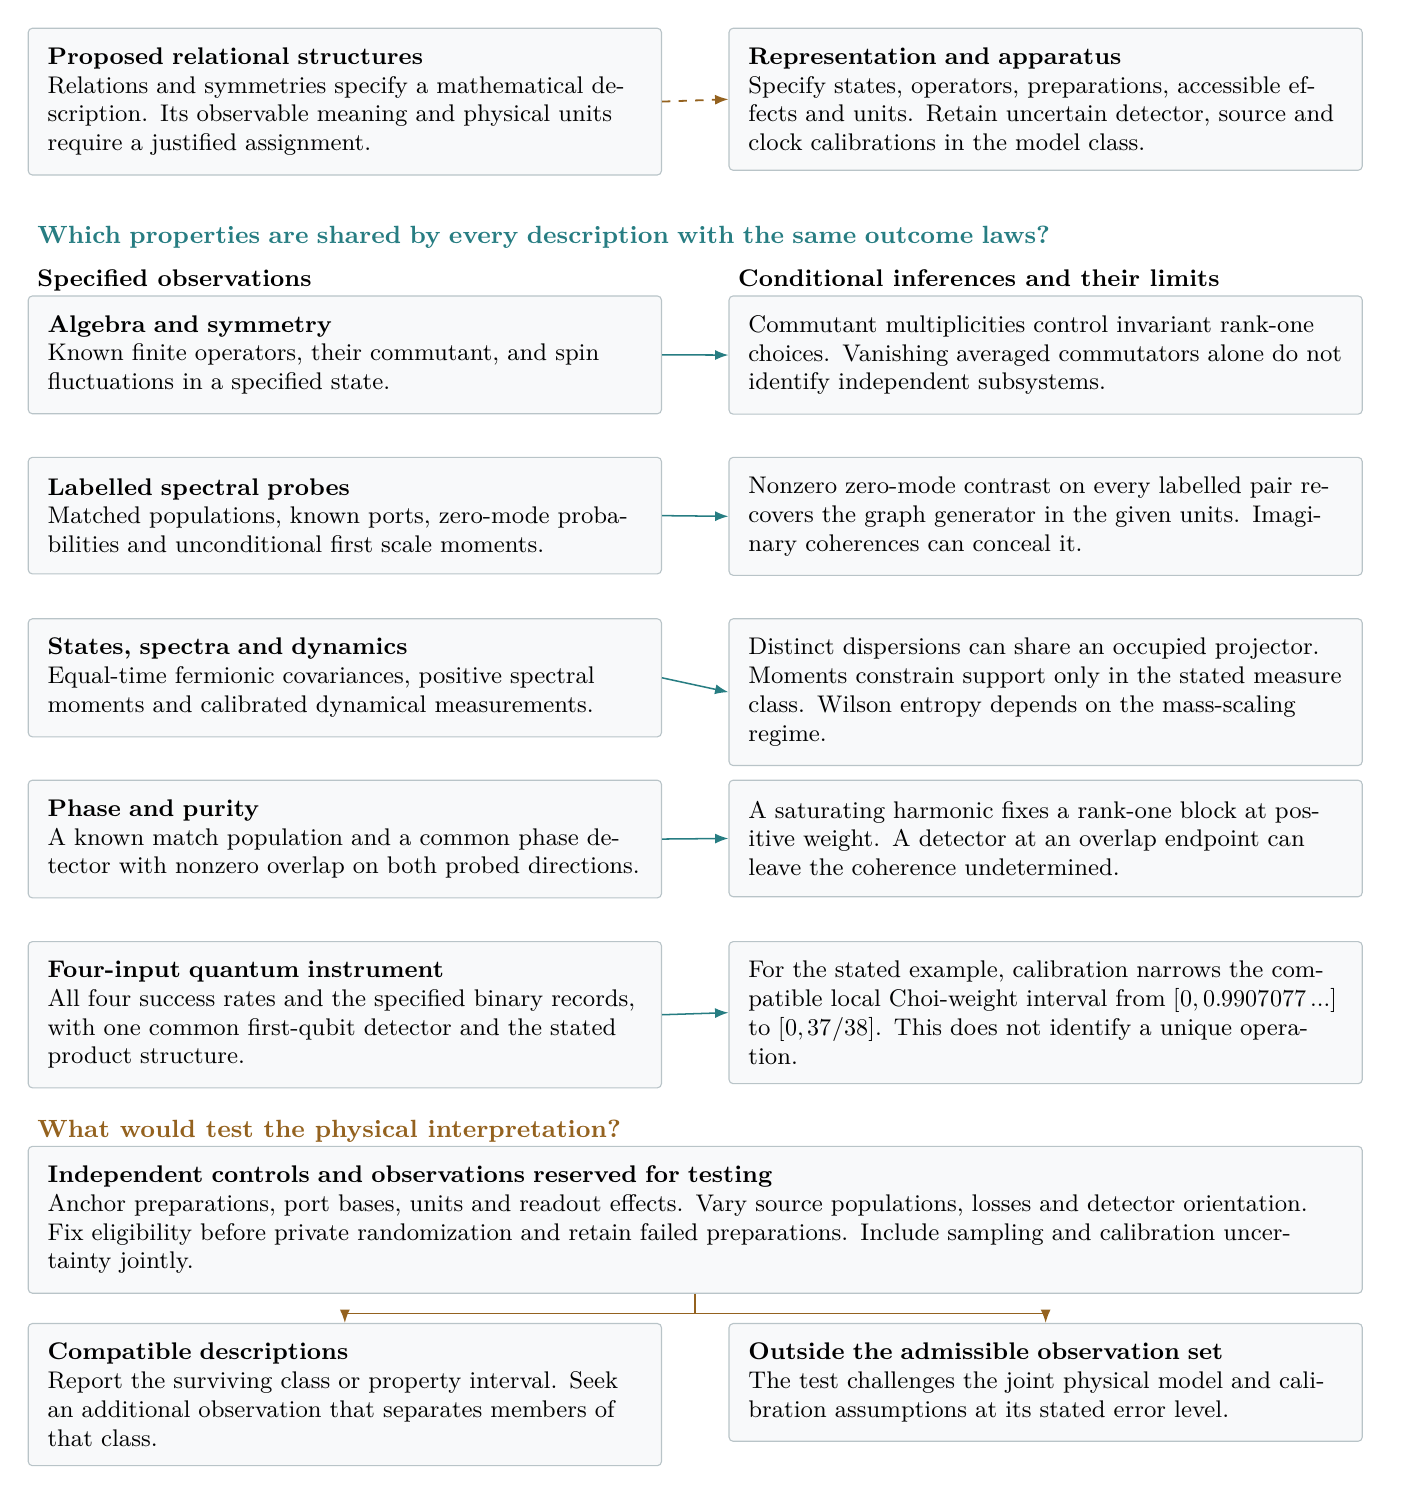
\begin{tikzpicture}[x=1cm,y=1cm,
 panel/.style={draw=ink!30,fill=ink!3,rounded corners=1.5pt,anchor=north west,
 text width=7.55cm,inner sep=7pt,align=left,font=\fontsize{8.7}{10.4}\selectfont},
 inference/.style={-{Latex[length=1.7mm]},draw=teal,line width=.55pt},
 open/.style={-{Latex[length=1.7mm]},draw=ochre,dashed,line width=.65pt}]
\node[panel,minimum height=1.65cm] (relations) at (0,0)
 {\textbf{Proposed relational structures}\par Relations and symmetries specify a mathematical description. Its observable meaning and physical units require a justified assignment.};
\node[panel,minimum height=1.65cm] (apparatus) at (8.9,0)
 {\textbf{Representation and apparatus}\par Specify states, operators, preparations, accessible effects and units. Retain uncertain detector, source and clock calibrations in the model class.};
\draw[open] (relations.east)--(apparatus.west);
\node[anchor=north west,text width=16.9cm,font=\small\bfseries\color{teal}] at (0,-2.40)
 {Which properties are shared by every description with the same outcome laws?};
\node[anchor=north west,font=\fontsize{8.7}{10.4}\selectfont\bfseries] at (0,-2.95) {Specified observations};
\node[anchor=north west,font=\fontsize{8.7}{10.4}\selectfont\bfseries] at (8.9,-2.95) {Conditional inferences and their limits};
\node[panel,minimum height=1.48cm] (algebra) at (0,-3.40)
 {\textbf{Algebra and symmetry}\par Known finite operators, their commutant, and spin fluctuations in a specified state.};
\node[panel,minimum height=1.48cm] (selection) at (8.9,-3.40)
 {Commutant multiplicities control invariant rank-one choices. Vanishing averaged commutators alone do not identify independent subsystems.};
\draw[inference] (algebra.east)--(selection.west);
\node[panel,minimum height=1.48cm] (spectra) at (0,-5.45)
 {\textbf{Labelled spectral probes}\par Matched populations, known ports, zero-mode probabilities and unconditional first scale moments.};
\node[panel,minimum height=1.48cm] (generator) at (8.9,-5.45)
 {Nonzero zero-mode contrast on every labelled pair recovers the graph generator in the given units. Imaginary coherences can conceal it.};
\draw[inference] (spectra.east)--(generator.west);
\node[panel,minimum height=1.48cm] (states) at (0,-7.50)
 {\textbf{States, spectra and dynamics}\par Equal-time fermionic covariances, positive spectral moments and calibrated dynamical measurements.};
\node[panel,minimum height=1.48cm] (dynamics) at (8.9,-7.50)
 {Distinct dispersions can share an occupied projector. Moments constrain support only in the stated measure class. Wilson entropy depends on the mass-scaling regime.};
\draw[inference] (states.east)--(dynamics.west);
\node[panel,minimum height=1.48cm] (phase) at (0,-9.55)
 {\textbf{Phase and purity}\par A known match population and a common phase detector with nonzero overlap on both probed directions.};
\node[panel,minimum height=1.48cm] (purity) at (8.9,-9.55)
 {A saturating harmonic fixes a rank-one block at positive weight. A detector at an overlap endpoint can leave the coherence undetermined.};
\draw[inference] (phase.east)--(purity.west);
\node[panel,minimum height=1.48cm] (instrument) at (0,-11.60)
 {\textbf{Four-input quantum instrument}\par All four success rates and the specified binary records, with one common first-qubit detector and the stated product structure.};
\node[panel,minimum height=1.48cm] (choi) at (8.9,-11.60)
 {For the stated example, calibration narrows the compatible local Choi-weight interval from $[0,0.9907077\ldots]$ to $[0,37/38]$. This does not identify a unique operation.};
\draw[inference] (instrument.east)--(choi.west);
\node[anchor=north west,font=\small\bfseries\color{ochre}] at (0,-13.75)
 {What would test the physical interpretation?};
\node[panel,text width=16.45cm,minimum height=1.45cm] (test) at (0,-14.20)
 {\textbf{Independent controls and observations reserved for testing}\par Anchor preparations, port bases, units and readout effects. Vary source populations, losses and detector orientation. Fix eligibility before private randomization and retain failed preparations. Include sampling and calibration uncertainty jointly.};
\node[panel,minimum height=1.48cm] (compatible) at (0,-16.45)
 {\textbf{Compatible descriptions}\par Report the surviving class or property interval. Seek an additional observation that separates members of that class.};
\node[panel,minimum height=1.48cm] (excluded) at (8.9,-16.45)
 {\textbf{Outside the admissible observation set}\par The test challenges the joint physical model and calibration assumptions at its stated error level.};
\coordinate (fork) at ($(test.south)+(0,-.25)$);
\draw[draw=ochre,line width=.55pt] (test.south)--(fork);
\draw[-{Latex[length=1.7mm]},draw=ochre,line width=.55pt] (fork)-|(compatible.north);
\draw[-{Latex[length=1.7mm]},draw=ochre,line width=.55pt] (fork)-|(excluded.north);
\end{tikzpicture}\par
\vspace{4mm}
{\small\textbf{Meaning of the arrows.} The dashed arrow marks an open physical correspondence. Solid horizontal arrows connect specified observations to conditional mathematical results. The lower branches are possible conclusions of a prospective test, not reported experimental outcomes. The five examples illustrate observation problems; they do not exhaust the program or constitute a derivation of a unique physical ontology.}\par
\vspace{3mm}
{\footnotesize\textbf{Sources.} K.~Justus, \emph{Identification from Restricted Measurements}; \emph{Operational Identification and Conditional Quantum Instruments}; \emph{Finite Part of Wilson--Dirac Relative Entropy}; and \emph{Uniform Modular Control and Nonlinear Convergence for Wilson--Dirac Intervals} (2026), in the accompanying \emph{Mathematical Supplement}.}
\end{document}
